%%%%%%%%%%%%%%%%%%%%%%%%%%%%%%%%%%%%%%%%%%%%%%%%%%%%%%%%%%%%
% File: hw.tex 						   %
% Description: LaTeX template for homework.                %
%
% Feel free to modify it (mainly the 'preamble' file).     %
% Contact hfwei@nju.edu.cn (Hengfeng Wei) for suggestions. %
%%%%%%%%%%%%%%%%%%%%%%%%%%%%%%%%%%%%%%%%%%%%%%%%%%%%%%%%%%%%

%%%%%%%%%%%%%%%%%%%%%%%%%%%%%%%%%%%%%%%%%%%%%%%%%%%%%%%%%%%%%%%%%%%%%%
% IMPORTANT NOTE: Compile this file using 'XeLaTeX' (not 'PDFLaTeX') %
%
% If you are using TeXLive 2016 on windows,                          %
% you may need to check the following post:                          %
% https://tex.stackexchange.com/q/325278/23098                       %
%%%%%%%%%%%%%%%%%%%%%%%%%%%%%%%%%%%%%%%%%%%%%%%%%%%%%%%%%%%%%%%%%%%%%%

\documentclass[11pt, a4paper, UTF8]{ctexart}
%%%%%%%%%%%%%%%%%%%%%%%%%%%%%%%%%%%
% File: preamble.tex
%%%%%%%%%%%%%%%%%%%%%%%%%%%%%%%%%%%

\usepackage[top = 1.5cm]{geometry}

% Set fonts commands
\newcommand{\song}{\CJKfamily{song}} 
\newcommand{\hei}{\CJKfamily{hei}} 
\newcommand{\kai}{\CJKfamily{kai}} 
\newcommand{\fs}{\CJKfamily{fs}}

\newcommand{\me}[2]{\author{{\bfseries 姓名:}\underline{#1}\hspace{2em}{\bfseries 学号:}\underline{#2}}}

% Always keep this.
\newcommand{\noplagiarism}{
  \begin{center}
    \fbox{\begin{tabular}{@{}c@{}}
      请独立完成作业,不得抄袭。\\
      若参考了其它资料,请给出引用。\\
      鼓励讨论,但需独立书写解题过程。
    \end{tabular}}
  \end{center}
}

% Each hw consists of three parts:
% (1) this homework
\newcommand{\beginthishw}{\part{作业}}
% (2) corrections (Optional)
\newcommand{\begincorrection}{\part{订正}}
% (3) any feedback (Optional)
\newcommand{\beginfb}{\part{反馈}}

% For math
\usepackage{amsmath}
\usepackage{amsfonts}
\usepackage{amssymb}

% Define theorem-like environments
\usepackage[amsmath, thmmarks]{ntheorem}

\theoremstyle{break}
\theorembodyfont{\song}
\theoremseparator{}
\newtheorem*{problem}{题目}

\theorempreskip{2.0\topsep}
\theoremheaderfont{\kai\bfseries}
\theoremseparator{:}
% \newtheorem*{remark}{注}
\theorempostwork{\bigskip\hrule}
\newtheorem*{solution}{解答}
\theorempostwork{\bigskip\hrule}
\newtheorem*{revision}{订正}

\theoremstyle{plain}
\newtheorem*{cause}{错因分析}
\newtheorem*{remark}{注}

\theoremstyle{break}
\theorempostwork{\bigskip\hrule}
\theoremsymbol{\ensuremath{\Box}}
\newtheorem*{proof}{证明}

\renewcommand\figurename{图}
\renewcommand\tablename{表}

% For figures
% for fig with caption: #1: width/size; #2: fig file; #3: fig caption
\newcommand{\fig}[3]{
  \begin{figure}[htp]
    \centering
      \includegraphics[#1]{#2}
      \caption{#3}
  \end{figure}
}

% for fig without caption: #1: width/size; #2: fig file
\newcommand{\fignocaption}[2]{
  \begin{figure}[htp]
    \centering
    \includegraphics[#1]{#2}
  \end{figure}
}  % modify this file if necessary
\usepackage{graphicx}
\usepackage{url}
\usepackage{float}

%%%%%%%%%%%%%%%%%%%%
\title{第二次作业:空间域与频率域滤波器}
\me{丁保荣}{171860509}
\date{\today}     % you can specify a date like ``2017年9月30日''.
%%%%%%%%%%%%%%%%%%%%
\begin{document}

\maketitle
%%%%%%%%%%%%%%%%%%%%

\section{从空间域滤波器生成频域滤波器}

\subsection{大致实现原理}
  sobel.m中包含了sobel算子的空间域滤波和频率域滤波。\par 
  average.m中包含了一个3*3的均值算子的空间域滤波和频率域滤波。\par 
  prewitt.m中包含了prewitt算子的空间域滤波和频率域滤波。\par
  laplacian.m中包含了一个$\alpha=0.2$的laplacian算子的空间域滤波和频率域滤波。\par 
  padding.m是用来实现补零操作的。\par 
  test.m是复现课程ppt中的代码的,做了一些改动。\par


 频域滤波器:首先对目标图像进行补零,中心化,然后进行傅里叶变换。对算子也进行类似操作。然后将傅里叶变换后的算子和傅里叶变换后的目标图像相乘,然后做傅里叶逆变换得到滤波后的图像。将新图像去中心化,取实部,并裁剪至原图像大小。我这里没有取abs,原因在后面会说明。\par 
 空间域滤波器:将算子和目标图像进行补零,然后进行卷积,然后将新图像裁剪至原图像大小。

 \subsection{实现效果}
原图如下所示:
\begin{figure}[H]
  \centering
  
  \begin{minipage}[t]{0.48\textwidth}
    \centering
    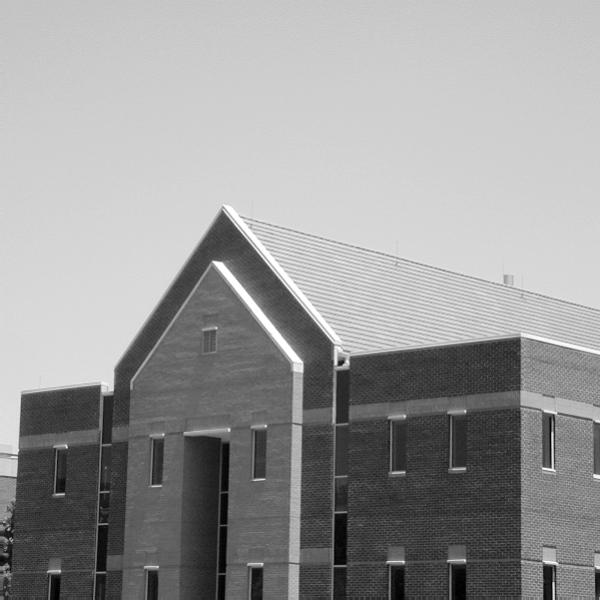
\includegraphics[width=7cm]{3_3.jpg}
    \caption{原图}
  \end{minipage}
  \begin{minipage}[t]{0.48\textwidth}
    \centering
    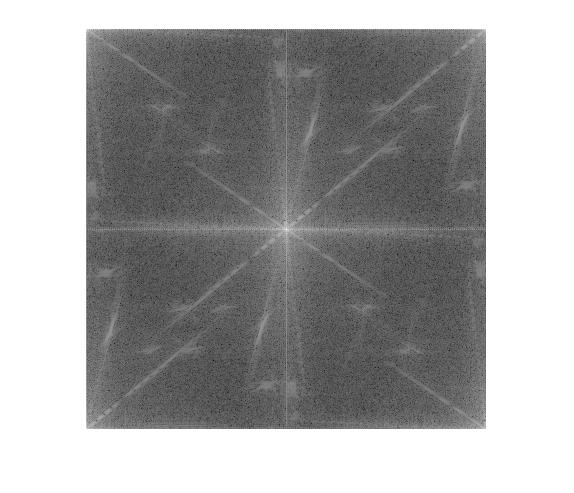
\includegraphics[width=7cm]{3_3_freq.jpg}
    \caption{原图的傅里叶谱}
  \end{minipage}  


\end{figure}


 \subsubsection{Sobel算子}
  \begin{figure}[H]
    \centering
    \begin{minipage}[t]{0.48\textwidth}
    \centering
    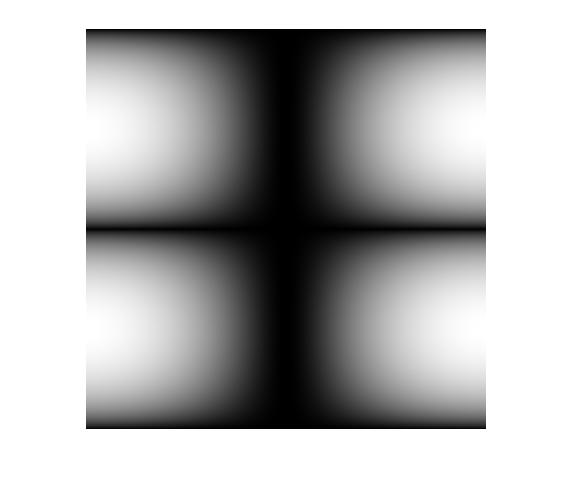
\includegraphics[width=7cm]{sobel.jpg}
    \caption{Sobel算子傅里叶谱}
    \end{minipage}
    \begin{minipage}[t]{0.48\textwidth}
    \centering
    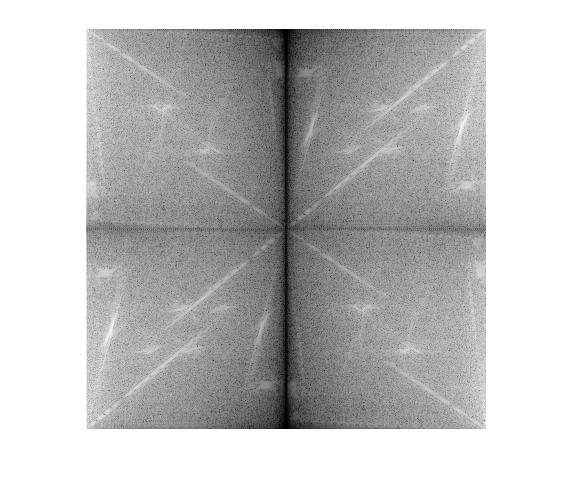
\includegraphics[width=7cm]{sobel_filter.jpg}
    \caption{原图经过sobel算子滤波后的傅里叶谱}
    \end{minipage}
  \end{figure}



  \begin{figure}[H]
    \centering
    \begin{minipage}[t]{0.48\textwidth}
    \centering
    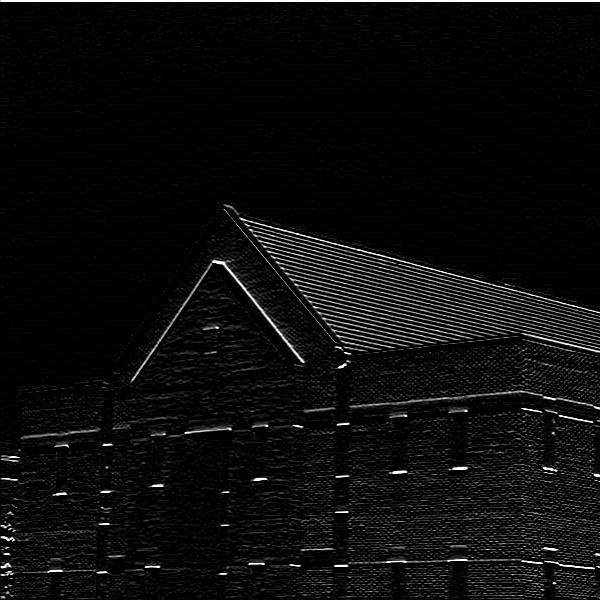
\includegraphics[width=7cm]{sobel_space.jpg}
    \caption{Sobel算子空间域滤波}
    \end{minipage}
    \begin{minipage}[t]{0.48\textwidth}
    \centering
    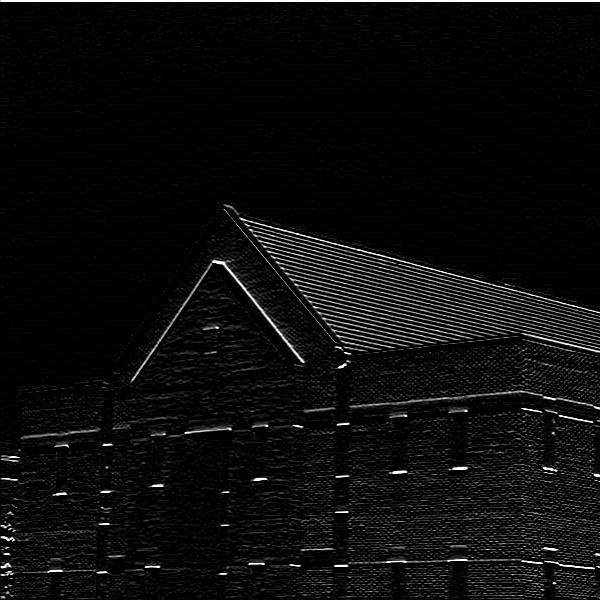
\includegraphics[width=7cm]{sobel_freq.jpg}
    \caption{Sobel算子频域滤波}
    \end{minipage}
  \end{figure}


  \subsubsection{均值算子}

  \begin{figure}[H]
    \centering
    \begin{minipage}[t]{0.48\textwidth}
    \centering
    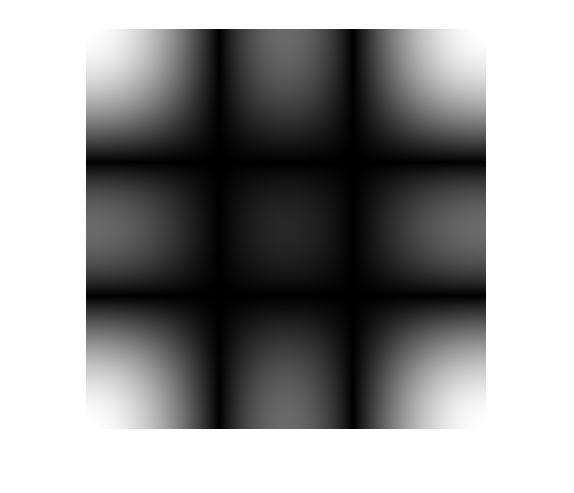
\includegraphics[width=7cm]{average.jpg}
    \caption{均值算子傅里叶谱}
    \end{minipage}
    \begin{minipage}[t]{0.48\textwidth}
    \centering
    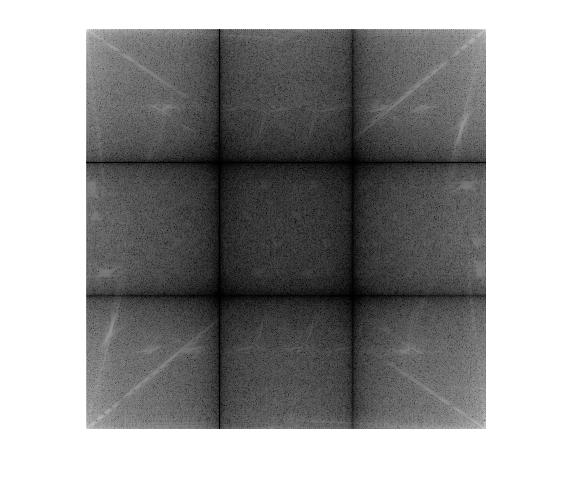
\includegraphics[width=7cm]{average_filter.jpg}
    \caption{原图经过均值算子滤波后的傅里叶谱}
    \end{minipage}
  \end{figure}




  \begin{figure}[H]
    \centering
    \begin{minipage}[t]{0.48\textwidth}
    \centering
    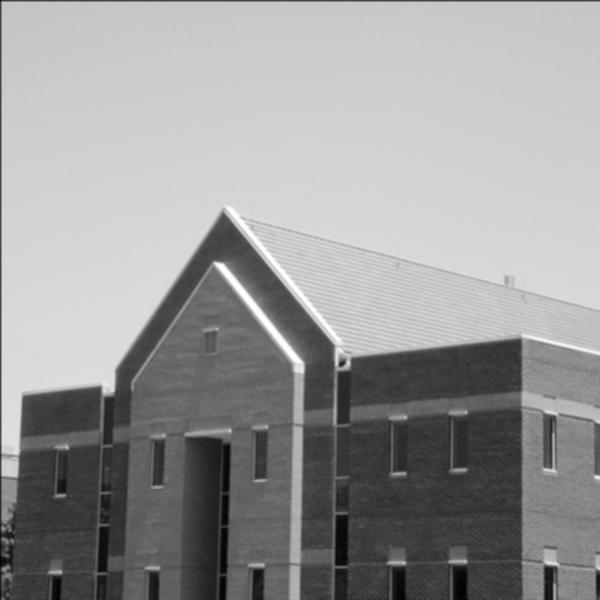
\includegraphics[width=7cm]{avg_space.jpg}
    \caption{3*3的均值算子空间域滤波}
    \end{minipage}
    \begin{minipage}[t]{0.48\textwidth}
    \centering
    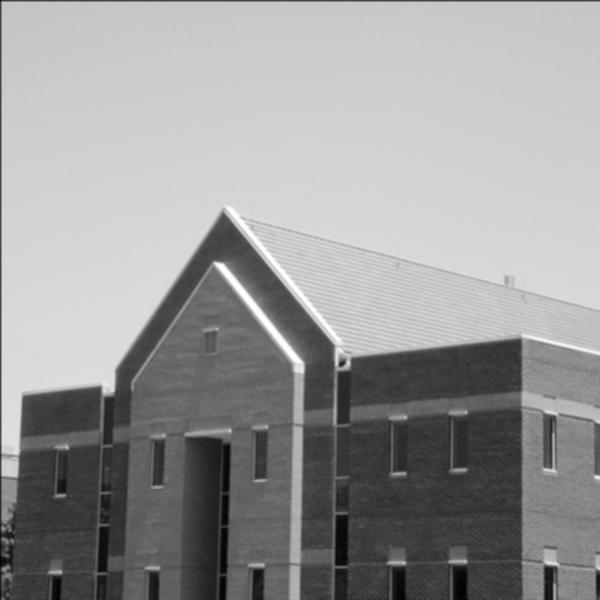
\includegraphics[width=7cm]{avg_freq.jpg}
    \caption{3*3的均值算子频域滤波}
    \end{minipage}
  \end{figure}

  \subsubsection{prewitt算子}

  \begin{figure}[H]
    \centering
    \begin{minipage}[t]{0.48\textwidth}
    \centering
    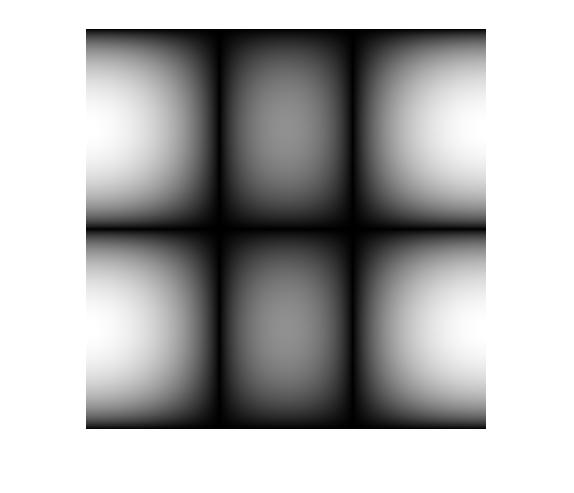
\includegraphics[width=7cm]{prewitt.jpg}
    \caption{prewitt算子傅里叶谱}
    \end{minipage}
    \begin{minipage}[t]{0.48\textwidth}
    \centering
    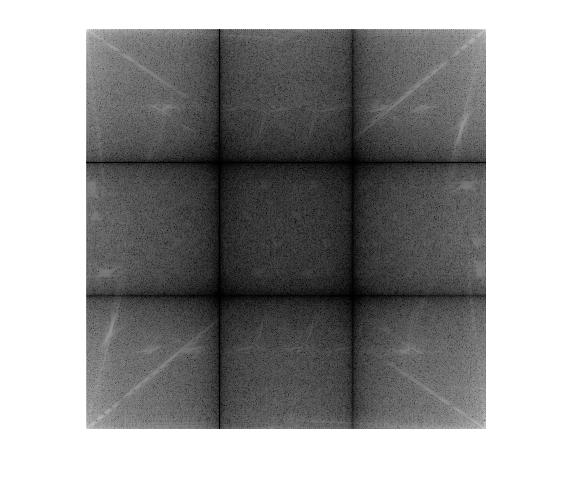
\includegraphics[width=7cm]{average_filter.jpg}
    \caption{原图经过prewitt算子滤波后的傅里叶谱}
    \end{minipage}
  \end{figure}



  \begin{figure}[H]
    \centering
    \begin{minipage}[t]{0.48\textwidth}
    \centering
    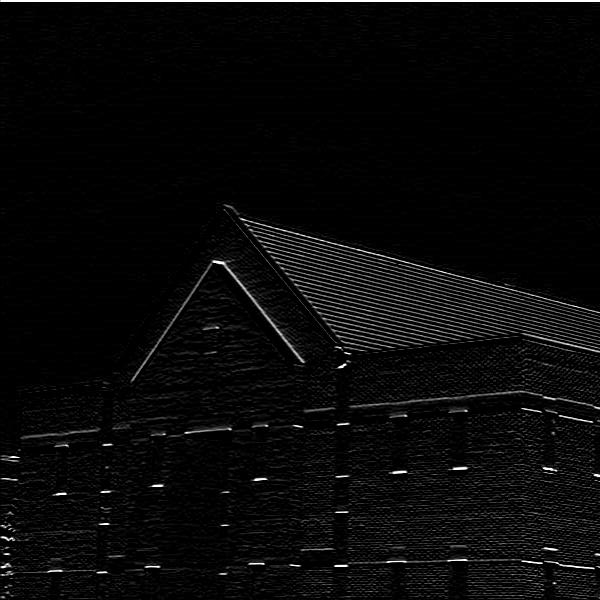
\includegraphics[width=7cm]{prewitt_space.jpg}
    \caption{prewitt算子空间域滤波}
    \end{minipage}
    \begin{minipage}[t]{0.48\textwidth}
    \centering
    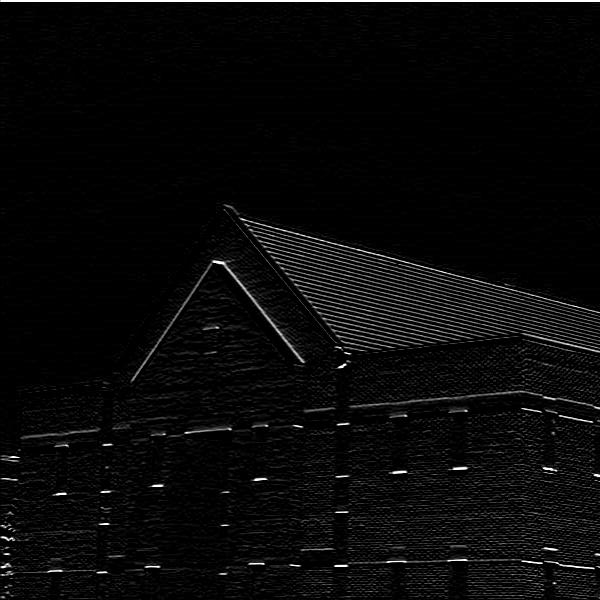
\includegraphics[width=7cm]{prewitt_freq.jpg}
    \caption{prewitt算子频域滤波}
    \end{minipage}
  \end{figure}

  \subsubsection{laplacian算子}

  \begin{figure}[H]
    \centering
    \begin{minipage}[t]{0.48\textwidth}
    \centering
    
\includegraphics[width=7cm]{laplacian.jpg}
    \caption{laplacian算子傅里叶谱}
    \end{minipage}
    \begin{minipage}[t]{0.48\textwidth}
    \centering
    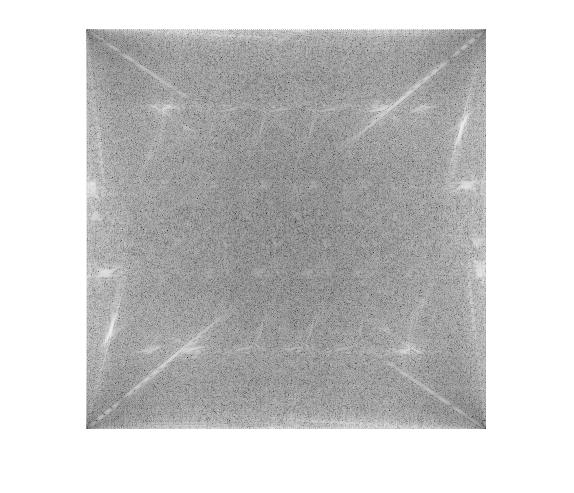
\includegraphics[width=7cm]{laplacian_filter.jpg}
    \caption{原图经过laplacian算子滤波后的傅里叶谱}
    \end{minipage}
  \end{figure}


  \begin{figure}[H]
    \centering
    \begin{minipage}[t]{0.48\textwidth}
    \centering
    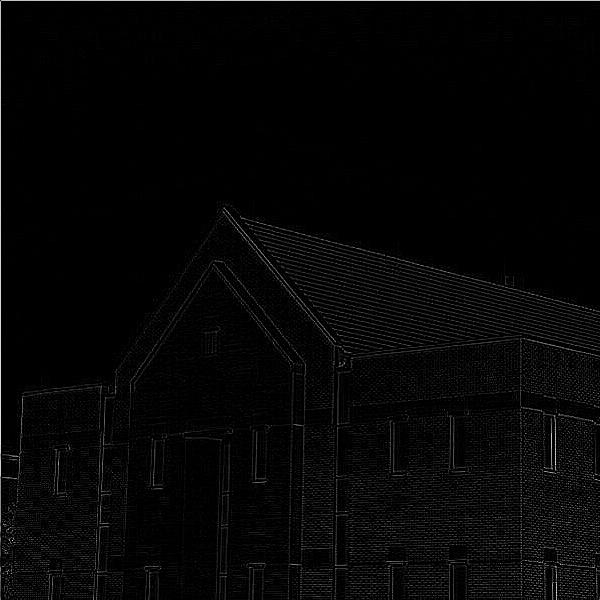
\includegraphics[width=7cm]{laplacian_space.jpg}
    \caption{$\alpha=0.2$的laplacian算子空间域滤波}
    \end{minipage}
    \begin{minipage}[t]{0.48\textwidth}
    \centering
    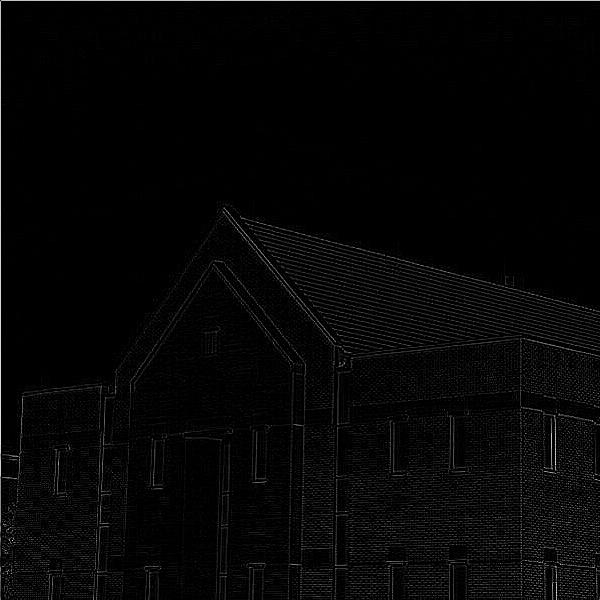
\includegraphics[width=7cm]{laplacian_freq.jpg}
    \caption{$\alpha=0.2$的laplacian算子频域滤波}
    \end{minipage}
  \end{figure}





\subsection{经验或教训}

    1. 在测试课件上的代码时,发现效果不对,最后发现课件上的代码没有把图像还原成原来的大小。\par 
    2. 显示图像的时候,要转换成uint8, 不然效果很奇怪。\par
    \begin{figure}[H]
      \centering
      \begin{minipage}[t]{0.48\textwidth}
      \centering
      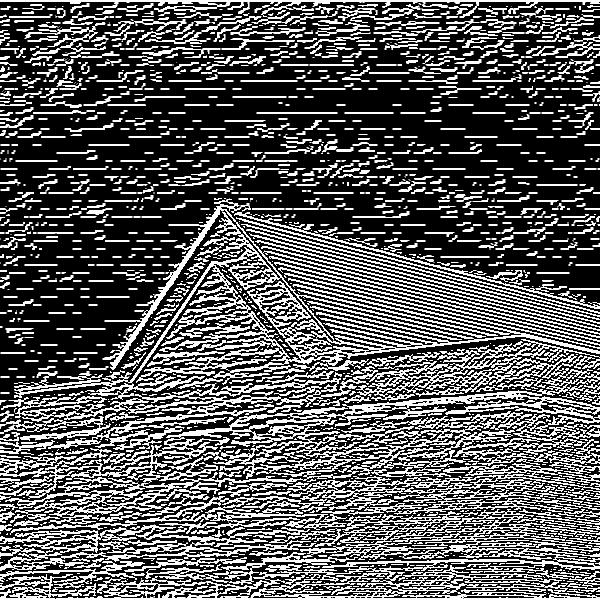
\includegraphics[width=7cm]{sobel_n_uint8.jpg}
      \caption{未进行类型转换}
      \end{minipage}
      \begin{minipage}[t]{0.48\textwidth}
      \centering
      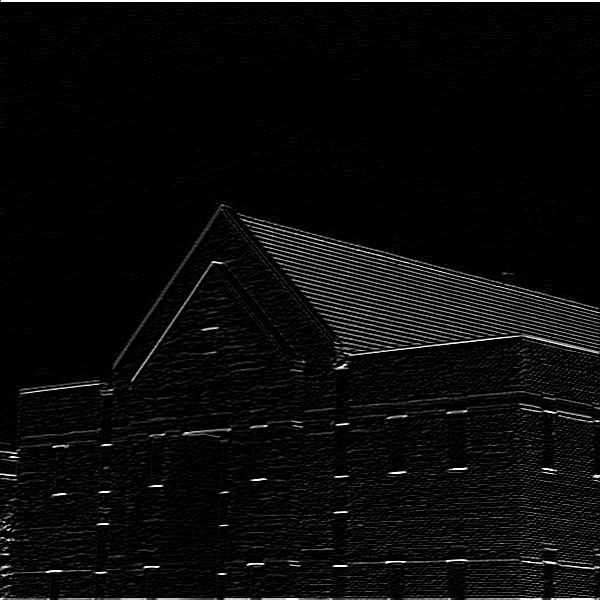
\includegraphics[width=7cm]{sobel_uint8.jpg}
      \caption{进行类型转换}
      \end{minipage}
    \end{figure}


    3. 我发现最后显示图像前,如果对图像取abs会发现错误,效果如下所示。注意看屋顶。\par 
    \begin{figure}[H]
      \centering
      \begin{minipage}[t]{0.48\textwidth}
      \centering
      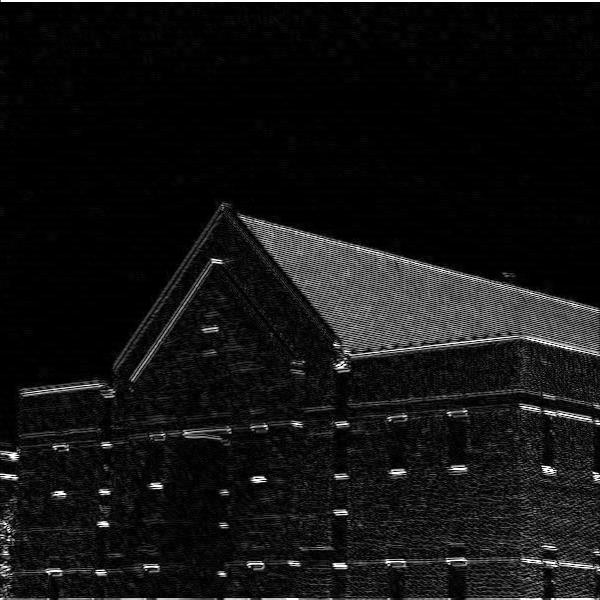
\includegraphics[width=7cm]{sobel_abs.jpg}
      \caption{使用abs函数}
      \end{minipage}
      \begin{minipage}[t]{0.48\textwidth}
      \centering
      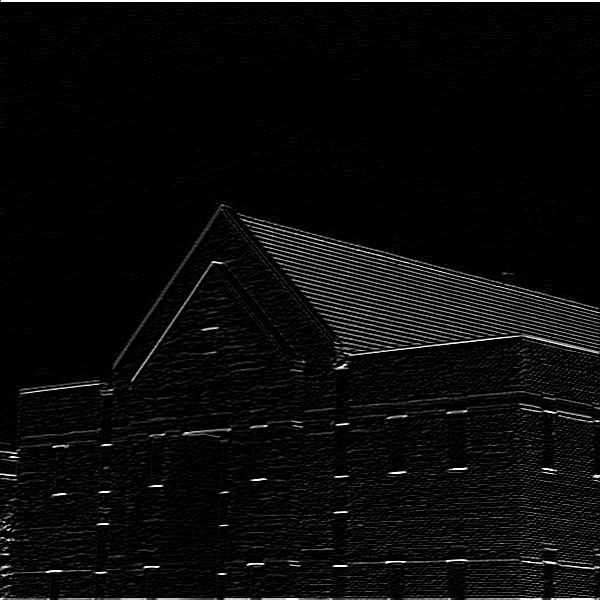
\includegraphics[width=7cm]{sobel_n_abs.jpg}
      \caption{不使用abs函数}
      \end{minipage}
    \end{figure}
    


    \section{美颜软件}

    \subsection{大致实现原理}
    log\_convertion.m文件里是一个对图像进行对数灰度变换的函数,公式如下,可以用来实现美白功能。\par 
    \begin{equation*}
        Output(i,j) = \frac{ \log{(Input(i,j) *(\beta-1) +1 )}}{\log{\beta}}
    \end{equation*}

    Butterworth.m文件中包含了巴特沃斯低通滤波器的实现。\par 
    GausLow.m文件中包含了高斯低通滤波器的实现。 \par 
    Ideal.m文件中包含了理想低通滤波器的实现。\par 
    midFilter.m文件中包含了中值滤波器的实现。\par 
    RF.m文件中包含了递归域变换滤波器的实现,代码参考自网络,并做了小幅修改。 \par


    主要实现的点在于生成相应的滤波器。首先对大小为$m \times n$ 的图像进行补零,形成大小为$2m \times 2n$的图像,并进行中心化。所以我们设计的滤波器大小为$2m \times 2n$, 且 中心位于$(m+1,n+1)$,所以我们可以对滤波器矩阵中的每个点,根据它与中心的距离按照公式来赋值即可。

    \subsection{实现效果}

    \subsection{理想低通滤波器}

    
    \begin{figure}[H]
      \centering
      \begin{minipage}[t]{0.48\textwidth}
      \centering
      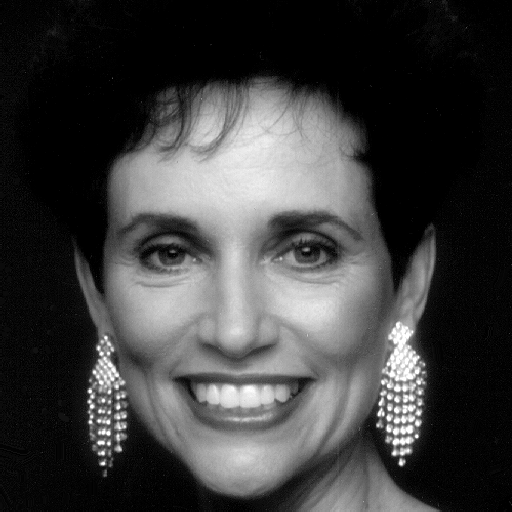
\includegraphics[width=7cm]{woman.png}
      \caption{原图}
      \end{minipage}
      \begin{minipage}[t]{0.48\textwidth}
      \centering
      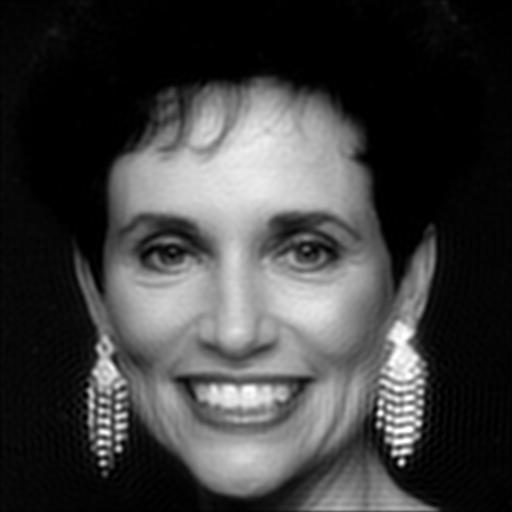
\includegraphics[width=7cm]{Ideal_130Hz.jpg}
      \caption{$D_0 =130Hz$}
      \end{minipage}
      \begin{minipage}[t]{0.48\textwidth}
        \centering
        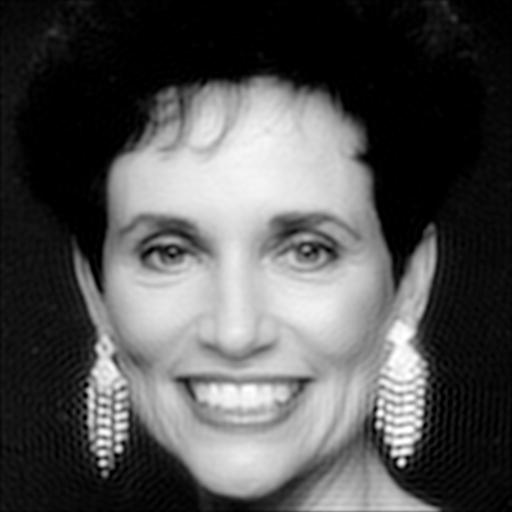
\includegraphics[width=7cm]{Ideal_log.jpg}
        \caption{加入美白效果,$\beta=5$}
        \end{minipage}
    \end{figure}
    可以看出理想滤波器对眼角的皱纹稍微去除了一点,但整个图像也变得有些模糊了,尤其是脸颊和脖子处。美白效果较好。



    \subsection{巴特沃斯低通滤波器}

    \begin{figure}[H]
      \centering
      \begin{minipage}[t]{0.48\textwidth}
      \centering
      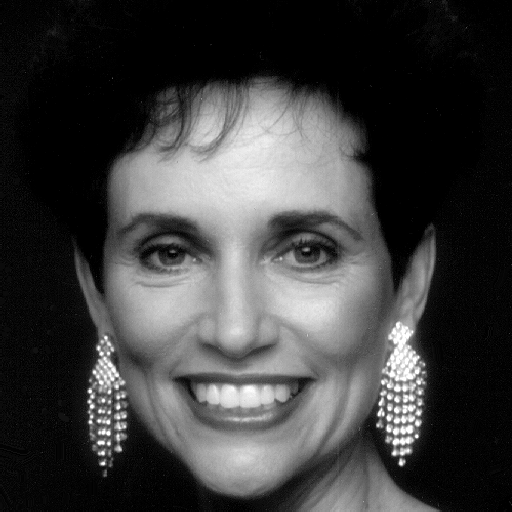
\includegraphics[width=7cm]{woman.png}
      \caption{原图}
      \end{minipage}
      \begin{minipage}[t]{0.48\textwidth}
      \centering
      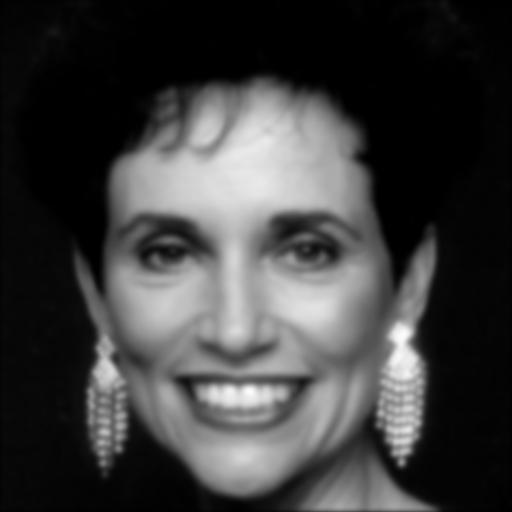
\includegraphics[width=7cm]{Bw_80Hz.jpg}
      \caption{$D_0 =80Hz,N=2$}
      \end{minipage}
      \begin{minipage}[t]{0.48\textwidth}
        \centering
        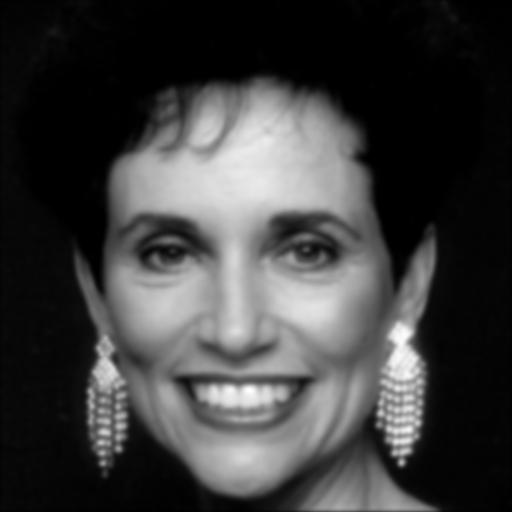
\includegraphics[width=7cm]{Bw_100Hz.jpg}
        \caption{$D_0 =100Hz,N=2$}
        \end{minipage}
      \begin{minipage}[t]{0.48\textwidth}
        \centering
        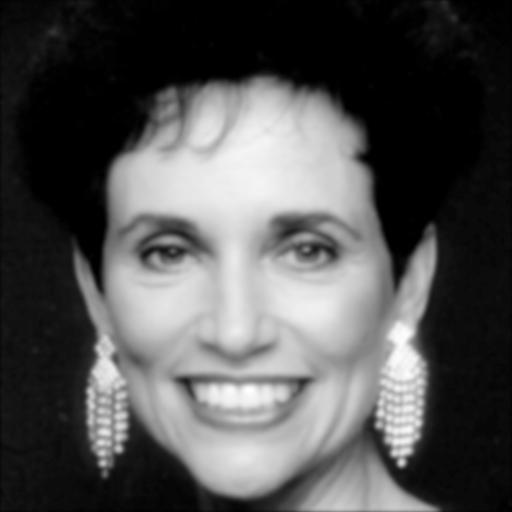
\includegraphics[width=7cm]{Bw_log.jpg}
        \caption{加入美白效果,$\beta=5$}
        \end{minipage}
    \end{figure}
    可以看出巴特沃斯低通滤波器的效果比理想滤波器的要好一点,$D_0 =100Hz$的效果较好。


    \subsection{高斯低通滤波器}

    \begin{figure}[H]
      \centering
      \begin{minipage}[t]{0.48\textwidth}
      \centering
      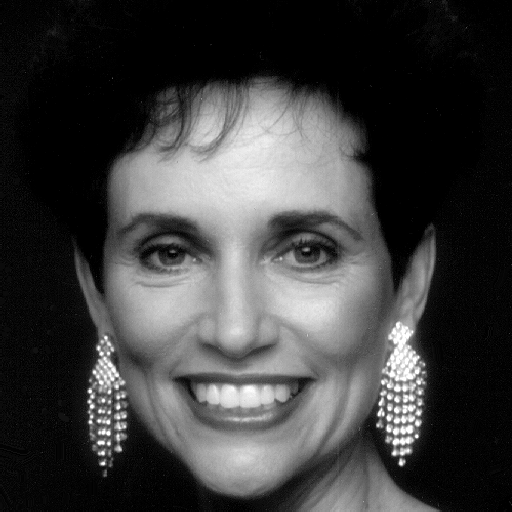
\includegraphics[width=7cm]{woman.png}
      \caption{原图}
      \end{minipage}
      \begin{minipage}[t]{0.48\textwidth}
      \centering
      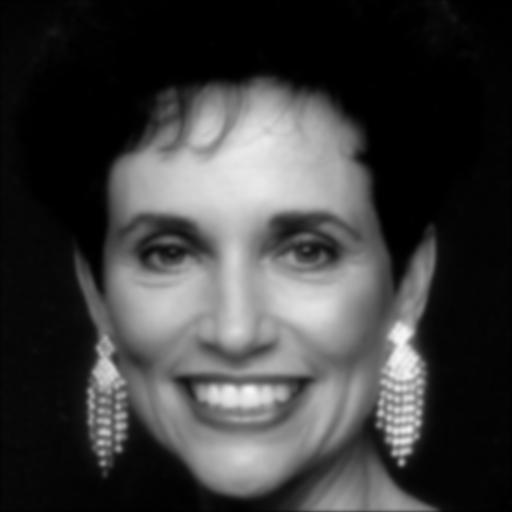
\includegraphics[width=7cm]{Gaus_80Hz.jpg}
      \caption{$D_0 =80Hz$}
      \end{minipage}
      \begin{minipage}[t]{0.48\textwidth}
        \centering
        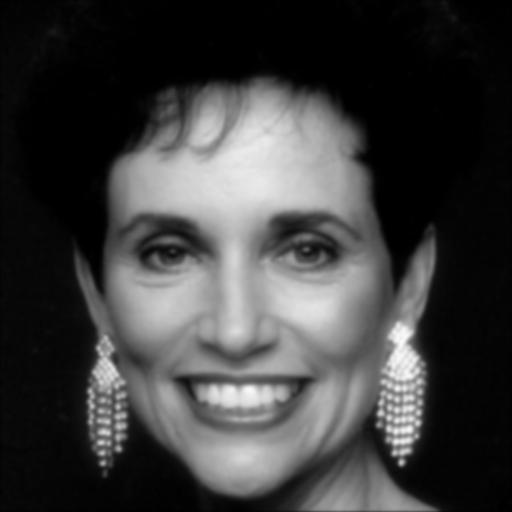
\includegraphics[width=7cm]{Gaus_100Hz.jpg}
        \caption{$D_0 =100Hz$}
        \end{minipage}
      \begin{minipage}[t]{0.48\textwidth}
        \centering
        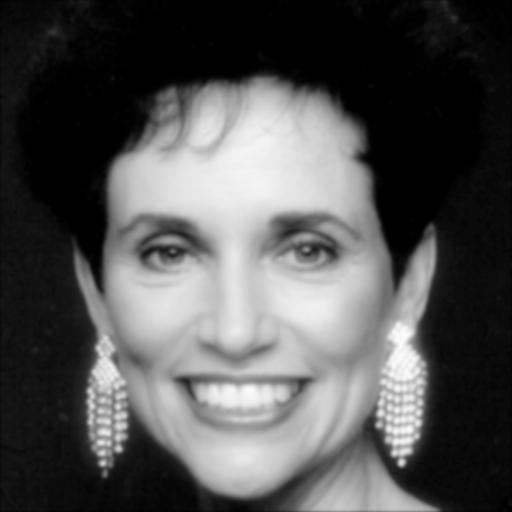
\includegraphics[width=7cm]{Gaus_log.jpg}
        \caption{加入美白效果,$\beta=5$}
        \end{minipage}
    \end{figure}

    \subsection{中值滤波器}

    \begin{figure}[H]
      \centering
      \begin{minipage}[t]{0.48\textwidth}
      \centering
      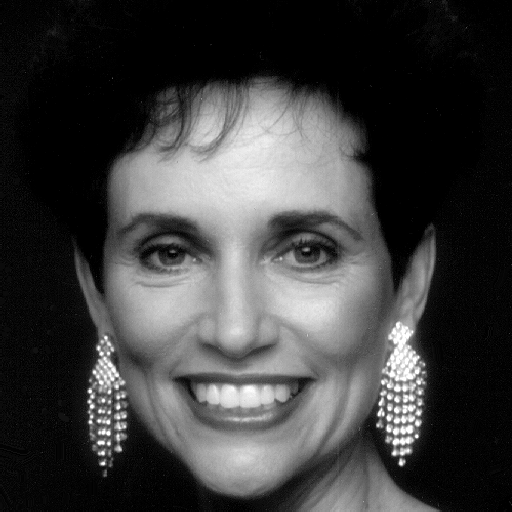
\includegraphics[width=7cm]{woman.png}
      \caption{原图}
      \end{minipage}
      \begin{minipage}[t]{0.48\textwidth}
      \centering
      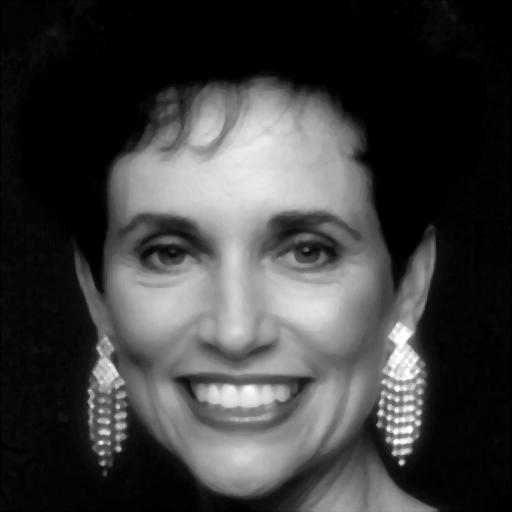
\includegraphics[width=7cm]{mid.jpg}
      \caption{大小为$5\times 5$的中值滤波器}
      \end{minipage}
      \begin{minipage}[t]{0.48\textwidth}
        \centering
        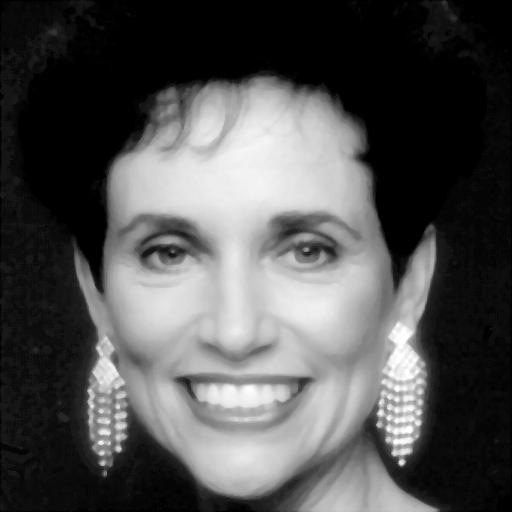
\includegraphics[width=7cm]{mid_log.jpg}
        \caption{加入美白效果,$\beta=5$}
        \end{minipage}
    \end{figure}



    \subsection{递归高斯滤波器}
    通过上面的几个滤波器,我们发现它们都会是图像变得很模糊,这是因为上面的几种滤波方法都都只考虑了空间邻近度,而忽视了像素之间的像素度。所以我在网上找到了另一类滤波叫做边缘保留滤波(Edge, Preserving Filter, EPF). EPF中有一个滤波叫做递归高斯滤波器(RF). 用它实现的效果较好。

    \begin{figure}[H]
      \centering
      \begin{minipage}[t]{0.48\textwidth}
      \centering
      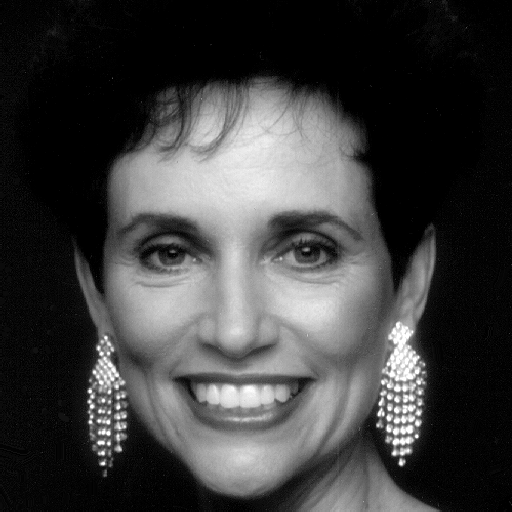
\includegraphics[width=7cm]{woman.png}
      \caption{原图}
      \end{minipage}
      \begin{minipage}[t]{0.48\textwidth}
      \centering
      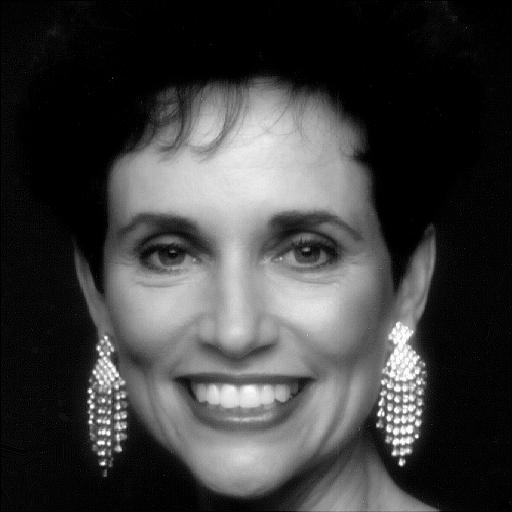
\includegraphics[width=7cm]{RF_30.jpg}
      \caption{透明度=30}
      \end{minipage}
      \begin{minipage}[t]{0.48\textwidth}
        \centering
        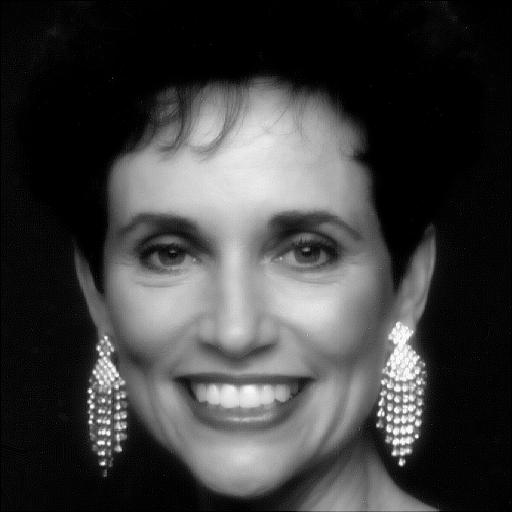
\includegraphics[width=7cm]{RF_50.jpg}
        \caption{透明度=50}
        \end{minipage}
      \begin{minipage}[t]{0.48\textwidth}
        \centering
        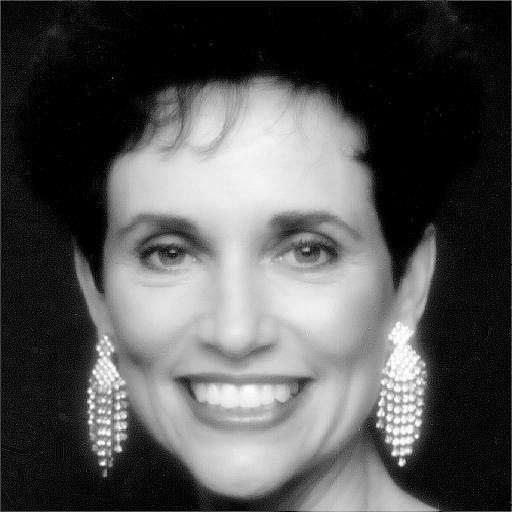
\includegraphics[width=7cm]{RF_log.jpg}
        \caption{加入美白效果,$\beta=5$}
        \end{minipage}
    \end{figure}







\end{document}